\documentclass[a4paper]{article}

\usepackage[utf8]{inputenc}
\usepackage[T1]{fontenc}
\usepackage{textcomp}
\usepackage[czech]{babel}
\usepackage{amsmath, amssymb}


% figure support
\usepackage{import}
\usepackage{xifthen}
\pdfminorversion=7
\usepackage{pdfpages}
\usepackage{transparent}
\newcommand{\incfig}[1]{%
    \def\svgwidth{\columnwidth}
    \import{./figures/}{#1.pdf_tex}
}

\pdfsuppresswarningpagegroup=1
\author{Hynek Kydlicek}
\title{Diskrétka 8}
\begin{document}
\maketitle
\section{Úkol 1 těžší verze}%
Z obr. \ref{fig:graf} vidíme, že graf je eulerovský a zároveň existuje hranově disjunktní rozklad na 3 a 2 kružnice.
\\
\subsection{3 kružnice}%
Kružnice jsou indukované podgrafy s vrcholy $\{1, 3, 4\}, \{1, 2, 5\}, \{2, 3, 6\}$.
\subsection{2 kružnice}%
Kružnice jsou indukovaný podgraf s vrcholy $\{1, 2, 3\}$ a graf s vrcholy $\{1, 5, 2, 6, 3, 4\}$ a hranami $\{1,5\}, \{5, 2\}, \{2, 6\}, \{6,3\}, \{3,4\}, \{4,1\}$.
\begin{figure}[htpb]
    \centering
    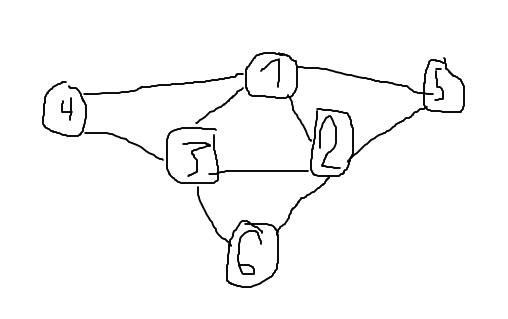
\includegraphics[width=0.8\textwidth]{graf.png}
    \caption{Graf}
    \label{fig:graf}
\end{figure}

\section{Úkol 2}
Stačí dokázat, že pro dva eulerovské grafy $G(V, E), H(V', E')$  je \mbox{$F= G \times H$} eulerovský.
Z definice pokud mezi vrcholy $v_1, v_2 \in V'$ vedla hrana v $V'$ povede hrana mezi vrcholy $(u \in V) \{(u, v_1), (u, v_2)\}$ v $F$.
Obdobně, pokud pokud mezi vrcholy $u_1, u_2 \in V$ vedla hrana v $V$ povede hrana mezi vrcholy $(v \in V') \{(v, u_1), (v, u_2)\}$ v $F$.
Celkově dostáváme že, do každého vrcholu $\{u, v\} \in F,\ u \in V,\  v \in V' $ povede tolik hrana kolik vedlo hran v $V$ do $u$ + kolik vedlo hran v $V'$ do $v$.
Jelikož jsou $G,H$ eulerovské, musí do každého vrcholu v $F$ vést sudý počet hran(sudé číslo + sudé číslo = sudé číslo).
Zároveň protože oba grafy $G,H$ jsou souvislé, musí být i $F$ souvislý. Mějme dva vrcholy z $(a_1, b_1), (a_2, b_2) \in F$.
Z definice a souvislosti $G$ víme, že existuje sled z $(a_1, b_1)$ do $(a_2, b_1)$.
Z definice a souvislosti $H$ víme, že existuje sled z $(a_2, b_1)$ do $(a_2, b_2)$.
Tedy spojením sledů dostáváme sled z $(a_1, b_1)$ do $(a_2, b_2)$.
Z přednášky víme, že existuje sled právě když existuje cesta a tedy $F$ je souvislý graf.
$F$ je proto eulerovské.

\end{document}
